\chapter{Experimental evaluation}
\label{ch:experiments}

This chapter shows the results of the experiments carried out to assess your contribution, usually compared to state of the art solutions. In the proposed structure, we separate experiments setup from experiment results, in which we list the experiments. This is especially convenient in case the setting is the same or very similar for all the experiments. Should this not be the case, you may consider instead to structure each experiment is a section/subsection and embed both setting and result inside it.

\begin{example}
In this chapter, we present experimental results on the algorithms proposed and we compare them with state of the art methods.
\end{example}

\section{Experimental setting}

First, describe the experimental setting. The setting usually contains:
\begin{itemize}
\item the dataset(s) used for the experiments;
\item the baselines, namely the other solutions with which you are comparing yours.
\end{itemize}

\begin{example}

\begin{table}[H]
\centering
\renewcommand{\arraystretch}{1.2}
\begin{tabular}{|l|c|c|c|c|c|}\hline
\textbf{Name}&$n$&$m$\\ \hline\hline
Email&1005&25571\\ \hline
\end{tabular}
\caption{Dataset used for the experiment.}
\label{tb:elf_datasets}
\end{table}

\paragraph{Datasets} \autoref{tb:elf_datasets} shows the characteristics of the real-world dataset used for the experiment. The dataset, provided by SNAP \cite{snapnets}, \emph{email-Eu-core}, has been generated using email data from a large European research institution. A directed edge $(u, v)$ means that person $u$ sent an e-mail to person $v$.

As widely done in literature, we assigned the ground-truth influence probabilities according to the weighted cascade model, that is, $p_{u,v}=\frac{1}{|In(v)|}$, for each edge $(u,v) \in E$.

\paragraph{Algorithms}

For the learning process, we use the Thompson Sampling (TS) as principal exploration strategy (\autoref{alg:cts}). For the sake of completeness, we show also results with a Pure Exploitation (PE) approach, in which the oracle is fed with the mean estimates of the influence probabilities at each round.

\end{example}

\section{Results}

In this section, we show and comment the results obtained from the experiments. Remember to comment every result and every figure you decide to insert in the thesis.

\begin{example}
\paragraph{Experiment 1}

\begin{figure}[H]
  \centering
  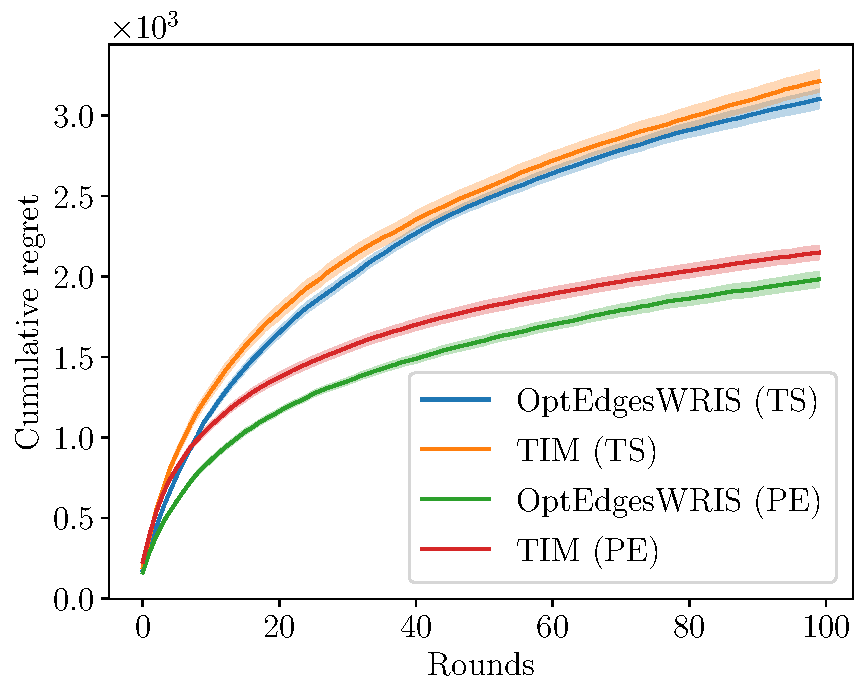
\includegraphics[width=.65\textwidth]{experiments/regret.pdf}
\caption{Cumulative regret in Email-In4 with 95\% confidence interval.}
\label{fig:exp_email}
\end{figure}

In this experiment, we test the algorithms on Email over a time horizon of $T=100$ rounds. The objective is to show the performances of the algorithms. The results have been averaged over 30 runs. \autoref{fig:exp_email} shows the cumulative regret, with a 95\% confidence interval.

As shown in the plot, our algorithm performs better with both the exploration strategies. However, the gain on TIM is more evident with the PE strategy, specially in the first rounds.
\end{example}